% Algorithm used to generate a QR code, to be included in architecture.tex

\subsubsection{QR code generator}
This section shows how QR codes can be generated in order to ensure security and meet other design decisions of the applications. The format of the string changes based on the type of the access request, but the suggested general form consists of
\begin{center}
	\texttt{control\_character + MD5(emissionDT + storeID + accessParam)}
\end{center}
Where the \texttt{control\_character} identifies the type of request through a number and the accessParam, exclusive to the type: 
\begin{itemize}[itemsep=-1mm, topsep=-1mm]
	\item Ticket:
	\begin{itemize}[itemsep=-1mm, topsep=-1mm]
		\item \texttt{control\_character}: 0
		\item \texttt{accessParam}: nOrder
	\end{itemize}
	\item Reservation:
	\begin{itemize}[itemsep=-1mm, topsep=-1mm]
		\item \texttt{control\_character}: 1
		\item \texttt{accessParam}: entranceTime 
	\end{itemize}			
\end{itemize}\vspace{.5\baselineskip}

Through the use of MD5 all codes are guaranteed to be of length 33 characters. Figure \ref{qr} shows an example of generated QR code for a ticket with parameters:
\begin{itemize}[itemsep=-1mm, topsep=-1mm]
	\item emissionDT: 2020-12-31 10:53:31 (without spaces and special characters)
	\item storeID: 154
	\item nOrder: 51
\end{itemize}\vspace{.5\baselineskip}
That corresponds to the string
\begin{center}
	\texttt{0dd8e72b69b8e4fac5c3f3bef07e09a4a}
\end{center}

\begin{figure}[h]	
	\centering
	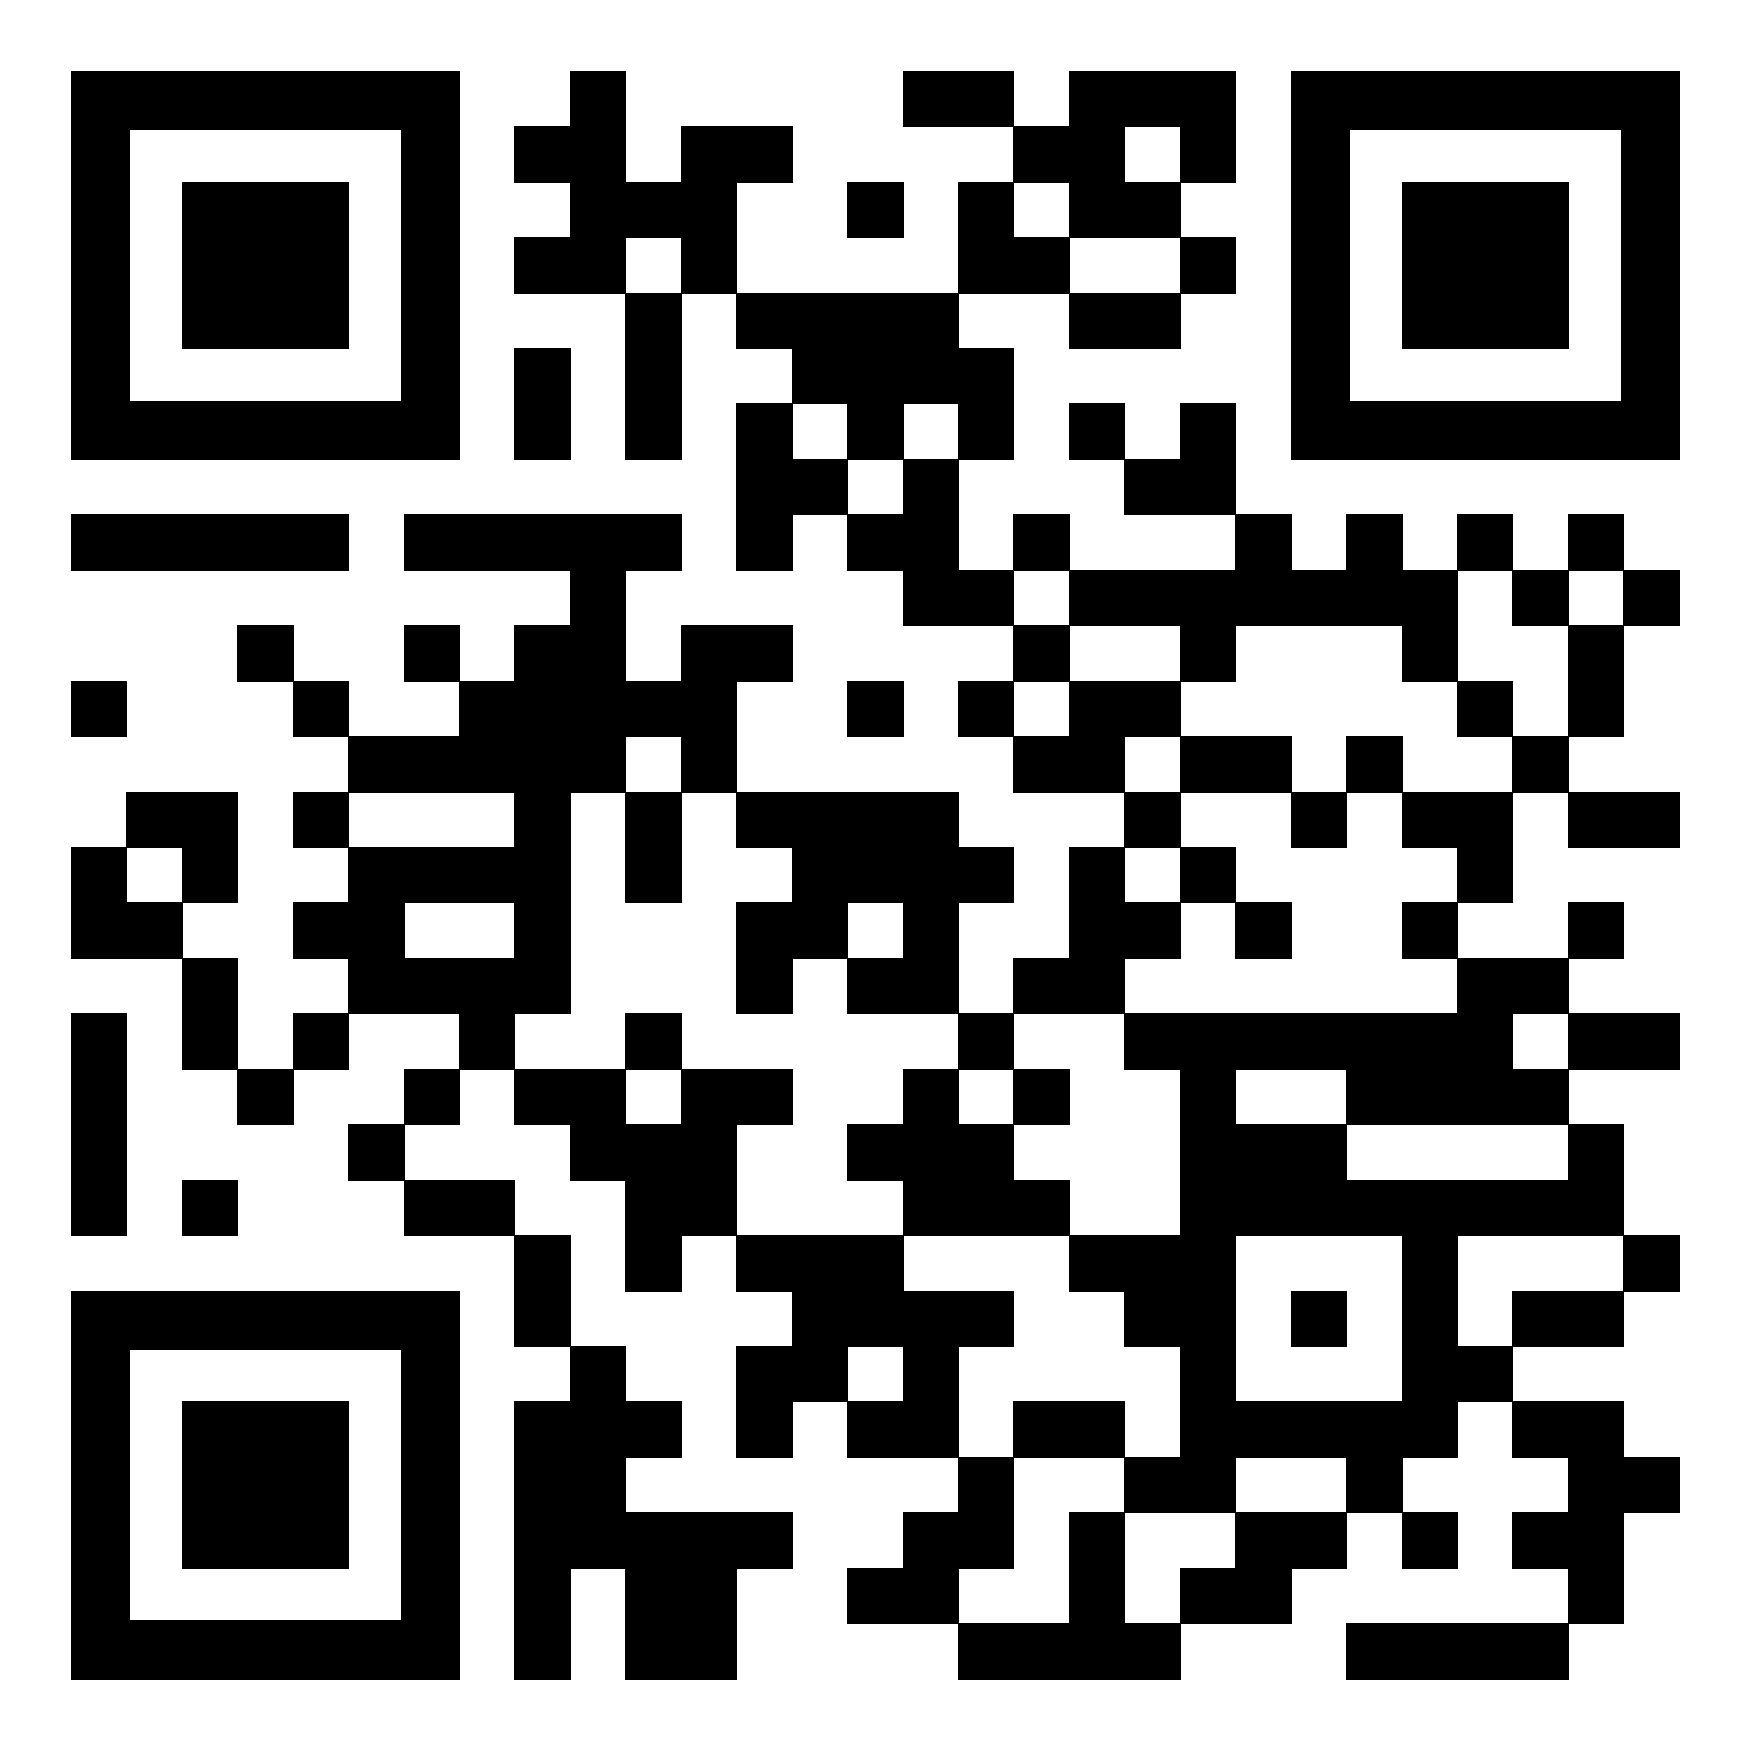
\includegraphics[width=.2\linewidth] {algorithms/qr-code}
	\caption{Generated QR code}
	\label{qr}
\end{figure}

 